%----------------------------------------------------------------------------------------
%    PACKAGES AND THEMES
%----------------------------------------------------------------------------------------

\documentclass[aspectratio=169,xcolor=dvipsnames]{beamer}
\usetheme{SimplePlus}

\usepackage{hyperref}
\usepackage{graphicx} % Allows including images
\usepackage{booktabs} % Allows the use of \toprule, \midrule and \bottomrule in tables

%----------------------------------------------------------------------------------------
%    TITLE PAGE
%----------------------------------------------------------------------------------------

%to remove slide counter
\setbeamertemplate{page number in head/foot}{}

\usepackage[backend=biber, style=authortitle]{biblatex}
\addbibresource{reference.bib}

\title{Newton's Method}
\subtitle{Solving Roots with Derivatives}

\author{Colby Cox}

\institute
{
    University of Central Arkansas % Your institution for the title page
}
\date{March 5, 2025} % Date, can be changed to a custom date

%----------------------------------------------------------------------------------------
%    PRESENTATION SLIDES
%----------------------------------------------------------------------------------------

\begin{document}

\begin{frame}
    % Print the title page as the first slide
    \titlepage
\end{frame}

% \begin{frame}{Overview}
%     % Throughout your presentation, if you choose to use \section{} and \subsection{} commands, these will automatically be printed on this slide as an overview of your presentation
%     \tableofcontents
% \end{frame}

%------------------------------------------------
% \section{First Section}
%------------------------------------------------

% \begin{frame}{Newton's Legacy}
%     We know Newton for his laws of physics, but he also was important in the discovery of Calculus and used it to describe what we call Newton's Method.
% \end{frame}

\begin{frame}{Quadratic Equation}
    \begin{itemize}
        \item[] <1->
        \begin{center}
            $ax^2 + bx + c = 0$
        \end{center}
        \item[] <2->
        \begin{center}
            $x = \frac{-b\pm \sqrt{b^2 - 4ac}}{2a}$
        \end{center}
    \end{itemize}
\end{frame}

\begin{frame}{Cubic Equation}
        \begin{itemize}
        \item[] <1-> 
        \begin{center}
            $ax^3 + bx^2 + cx + d = 0$
        \end{center}
        \item[] <2->
        \begin{center}
            $x = \sqrt[3]{\left( \frac{-b^3}{27a^3} + \frac{bc}{6a^2} + \frac{d}{2a} \right) + \sqrt{ \left( \frac{-b^3}{27a^3} + \frac{bc}{6a^2} - \frac{d}{2a} \right)^2 + \left( \frac{c}{3a} - \frac{b^2}{9a^2}\right)^3}} +  \sqrt[3]{\left( \frac{-b^3}{27a^3} + \frac{bc}{6a^2} - \frac{d}{2a} \right) - \sqrt{ \left( \frac{-b^3}{27a^3} + \frac{bc}{6a^2} - \frac{d}{2a} \right)^2 + \left( \frac{c}{3a} - \frac{b^2}{9a^2} \right)^3}} - \frac{b}{3a}$ \\
            %\cite{CubicEquation}
        \end{center}
    \end{itemize}
\end{frame}

\begin{frame}{Quartic Equation}
    \begin{center}
    \begin{itemize}
        \centering
        \item[] <1- > {$ax^4 + bx^3 + cx^2 + dx + e = 0$}
        \item[] <2- > {
        \only<2> {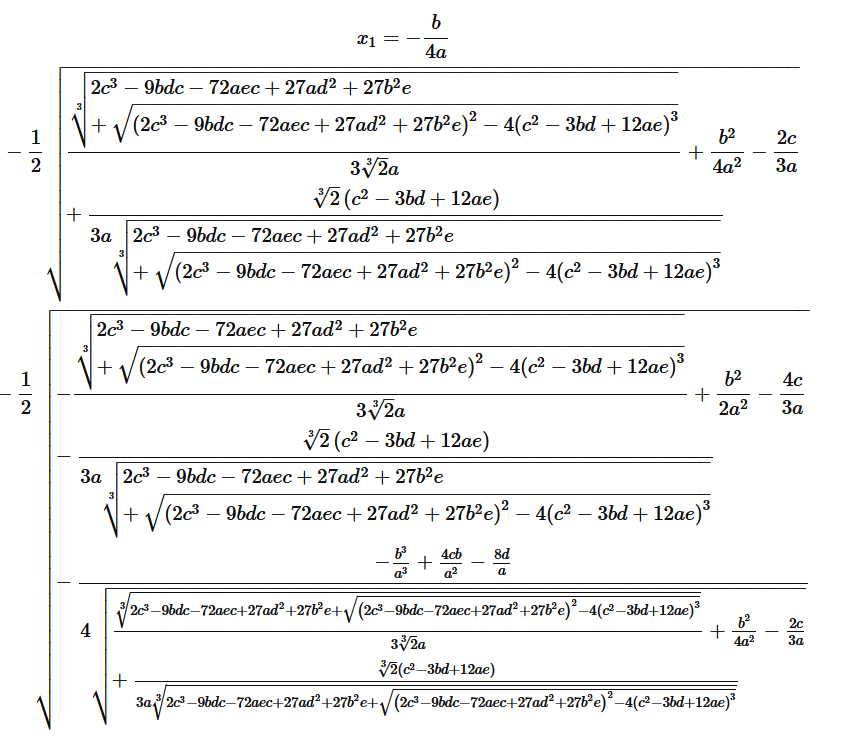
\includegraphics[scale=0.3]{images/x1.png}}
        \only<3> {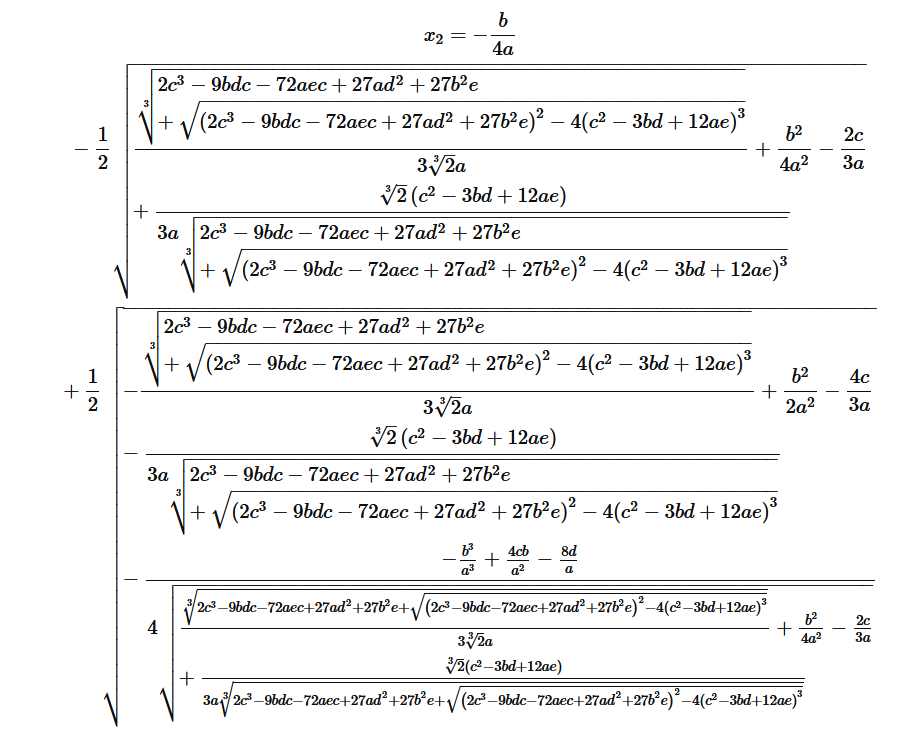
\includegraphics[scale=0.3]{images/x2.png}}
        \only<4> {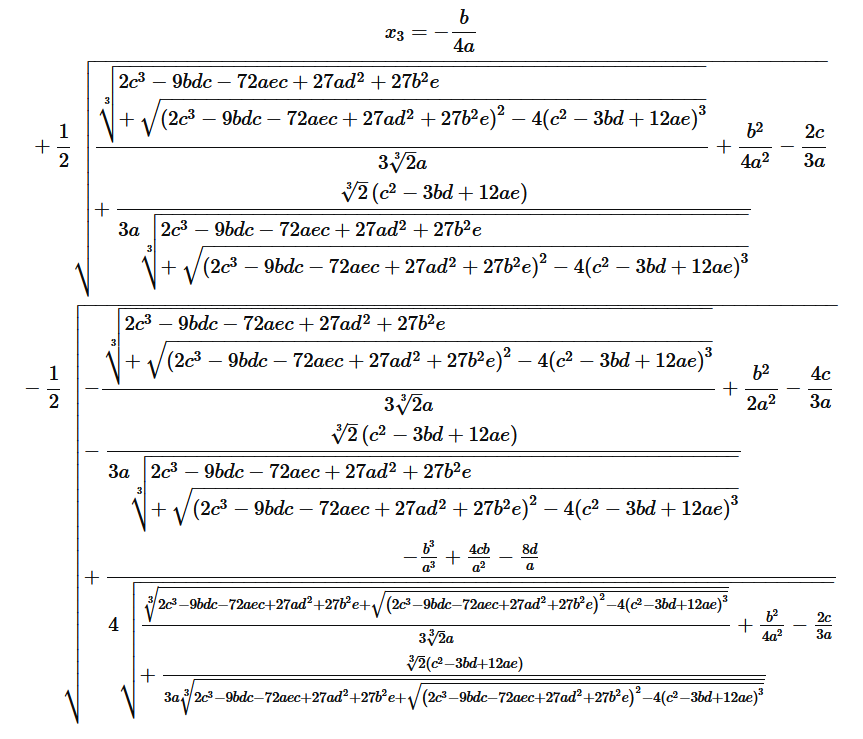
\includegraphics[scale=0.3]{images/x3.png}}
        \only<5> {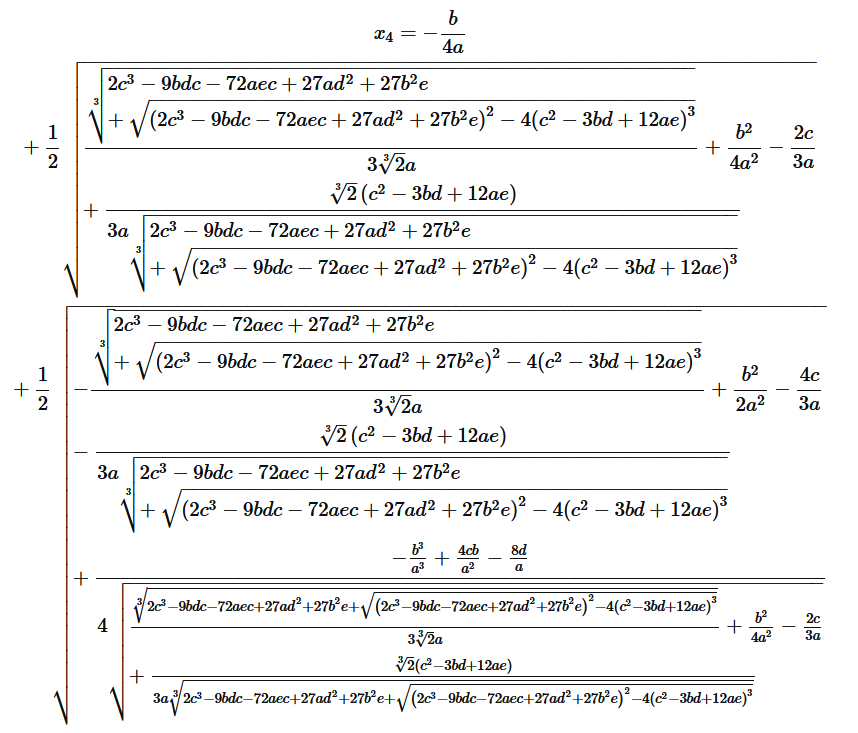
\includegraphics[scale=0.3]{images/x4.png}\vspace{0.3cm}}
        
        %\cite{QuarticEquation}
        }
        \end{itemize}
    \end{center}
\end{frame}

\begin{frame}{Quintic Equation}
    \begin{itemize}
        \centering
        \item[]<1-> $ax^5 + bx^4 + cx^3+dx^2+ex+f = 0$ \vspace{0.5cm}
        \item[]<2-> \Huge There is no quintic equation
    \end{itemize}
\end{frame}

\begin{frame}{Solving a Quintic Equation}
    \begin{itemize}
        \centering
        \item[]<1-> $f(x) = x^5-5x+3 = 0$
        \item[]<2-> $f'(x) = 5x^4-5, x_0 = 2$
        \begin{gather*}
            x_1 = x_0 - \frac{f(x_0)}{f'(x_0)} = 2 - \frac{25}{75} = 1.667
        \end{gather*}
        \item[]<3->
        \begin{gather*}
            x_2 = 1.443, x_3 = 1.32 , x_4 = 1.28 \\
            x_5 = 1.276, x_6 = 1.276, x_7 = 1.276
        \end{gather*}
    \end{itemize}
\end{frame}

\begin{frame}{Newton's Method}
    \begin{center}
        \Huge $x_{k+1} = x_k - \frac{f(x_k)}{f'(x_k)}$
    \end{center}
    \begin{itemize}
        \item $x_k$: Our current guess for the root
        \item $x_{k+1}$: Our next guess for the root
    \end{itemize}
\end{frame}

\begin{frame}{Tolerance}
    Tolerance is extremely dependent on the application you are designing for. For example: \\ \vspace{0.3cm}
    \begin{columns}
        \column{0.5\textwidth}
        \begin{center}
            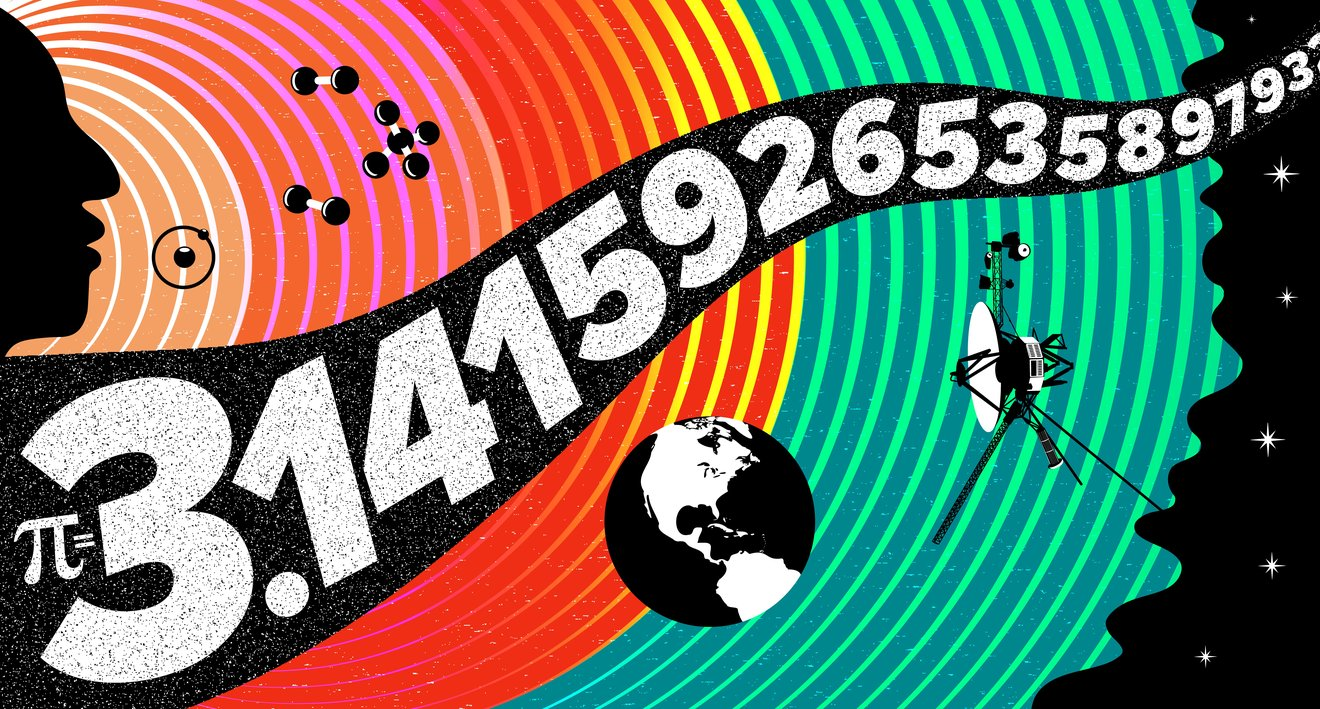
\includegraphics[scale=0.1]{images/piNasa.jpg} \\
            \small
            38 digits of $\pi$ is sufficient to calculate the circumference of the universe. \\ \vspace{0.1cm}
            \tiny
            %\cite{piNasa}
        \end{center}
        \column{0.5\textwidth}
        \begin{center}
            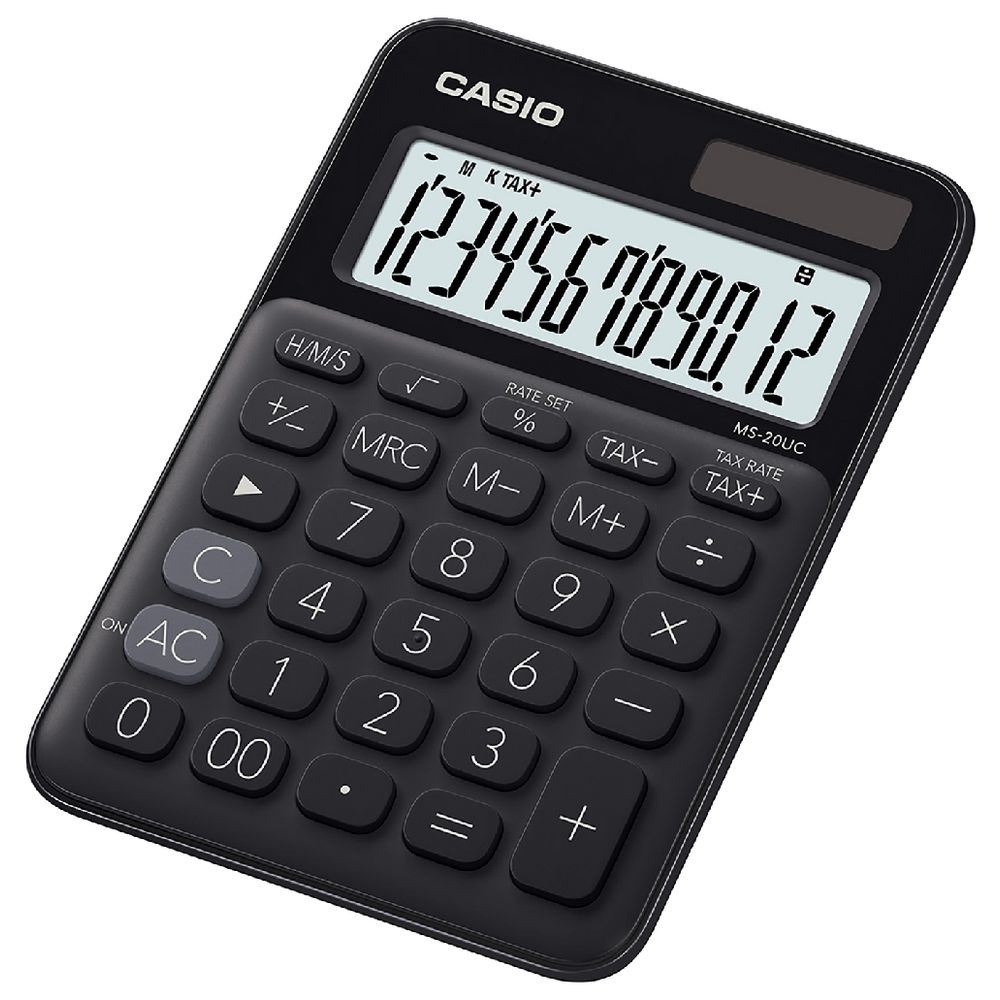
\includegraphics[scale=0.09]{images/calculator.jpg} \\
            \small
            We only need to calculate as many digits we can see on a calculator.
        \end{center}
    \end{columns}
\end{frame}

\begin{frame}{Square Root}
\begin{itemize}
    \item[]<1->
    \begin{center}
        Use Newton's Method to find any square root. \\
    \end{center}
    Let $\sqrt{a} = x$.
    \begin{gather*}
        a = x^2, x^2 - a = 0
    \end{gather*}
    \item[]<2->
    Let $f(x) = x^2 - a$.
    \begin{gather*}
        f'(x) = 2x
    \end{gather*}
    \item[]<3->
    Plug in to Newton's Method:
    \begin{gather*}
        x_{k+1} = x_k - \frac{x_k^2 - a}{2x_k} = \frac{1}{2} \left( x_k-\frac{a}{x_k} \right) \\
    \end{gather*}
\end{itemize}
\end{frame}

\begin{frame}{Solving a Square Root}
\begin{itemize}
\item[]<1->
    \begin{center}
        Using Newton's Method to solve $\sqrt{16}$. \vspace{0.3cm}
    \end{center}
    Let's choose an initial guess of 16 and a tolerance of 0.001
    \begin{gather*}
        f(x) = x^2 - 16, x_0 = 16 \\
        x_{1} = \frac{1}{2}\left( 16 - \frac{16}{16} \right) = 8.5 \\
        |8.5 - 16| = 7.5 \nless 0.001
    \end{gather*}
\item[]<2->
    Now let's use 8.5 as our $x_k$
    \begin{gather*}
        x_{2} = \frac{1}{2}\left( 8.5 - \frac{16}{8.5} \right) = 5.191 \\
        |5.191 - 8.5| = 3.3088 \nless 0.001
    \end{gather*}
    Let's continue iterating until the tolerance is satisfied
\end{itemize}
\end{frame}

\begin{frame}{Solving a Square Root}
    \begin{center}
        Using Newton's Method to solve $\sqrt{16}$
    \end{center}
    \begin{gather*}
        x_{3} = \frac{1}{2}\left( 5.191 - \frac{16}{5.191} \right) = 4.136664 \\
        |4.136664 - 5.191| = 1.0545 \nless 0.001 \\ \\
        x_{4} = \frac{1}{2}\left( 4.136664 - \frac{16}{4.136664} \right) = 4.0022... \\
        |4.136664 - 4.0022| = 0.1344 \nless 0.001 \\ \\
        x_{5} = \frac{1}{2}\left( 4.022 - \frac{16}{4.022} \right) = 4.0000006367 \\
        |4.022 - 4.0000006367| = 0.002 \nless 0.001
    \end{gather*}
\end{frame}

\begin{frame}{Solving a Square Root}
    \begin{center}
        Using Newton's Method to solve $\sqrt{16}$
    \end{center}
    \begin{gather*}
        x_{6} = \frac{1}{2}\left( 4.0000006367 - \frac{16}{4.0000006367} \right) = 4 \\
        |4 - 4.0000006367| = 6.367\times10^{-7} < 0.001 \\
    \end{gather*}
    \begin{center}
        So $\sqrt{16} = 4$
    \end{center}
\end{frame}

\begin{frame}{nth Root}
    \begin{center}
        Use Newton's Method to find the nth root. \\
    \end{center}
    Let $\sqrt[n]{a} = x$.
    \begin{gather*}
        a = x^n, x^n - a = 0
    \end{gather*}
    Let $f(x) = x^n - a$.
    \begin{gather*}
        f'(x) = nx^{n-1}
    \end{gather*}
    Plug in to Newton's Method:
    \begin{gather*}
        x_{k+1} = x_k - \frac{x_k^n - a}{nx_k^{n-1}} = \frac{1}{n} \left( x_k(n-1)+\frac{a}{x_k^{n-1}} \right) \\
    \end{gather*}
\end{frame}

\begin{frame}{Leetcode Problem}
    \begin{center}
        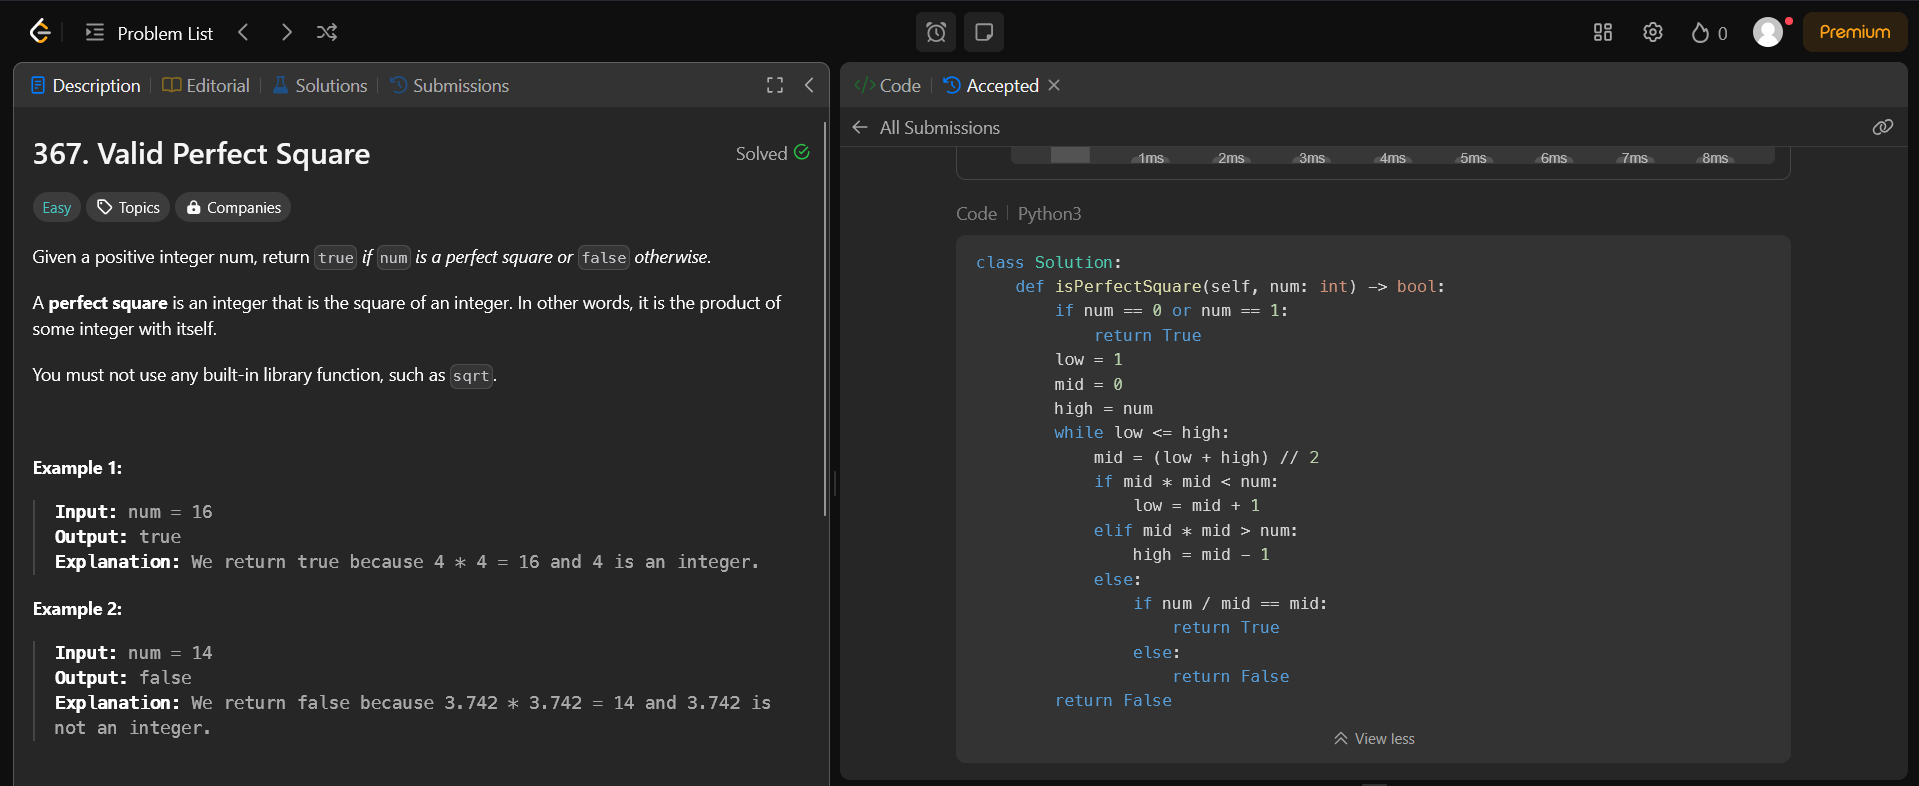
\includegraphics[scale=0.27]{images/leetcode.png}
    \end{center}
\end{frame}

\begin{frame}{Binary Search}
    \centering
    \only<1>
    {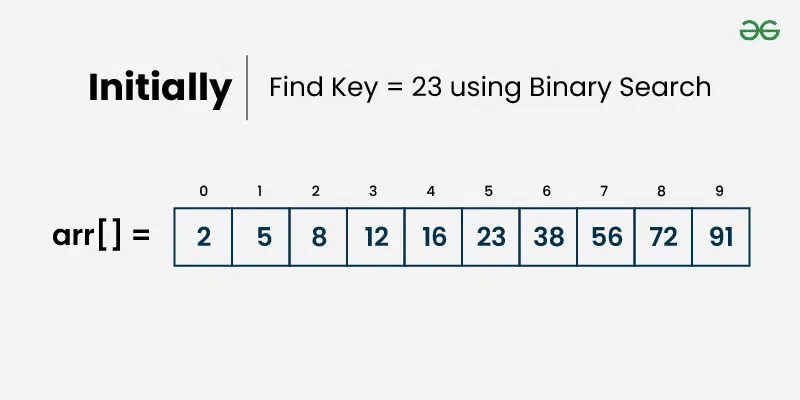
\includegraphics[scale=0.4]{images/Binary-Search-1.png} \\
    %\cite{BinarySearchGeeks}
    }
    \only<2>
    {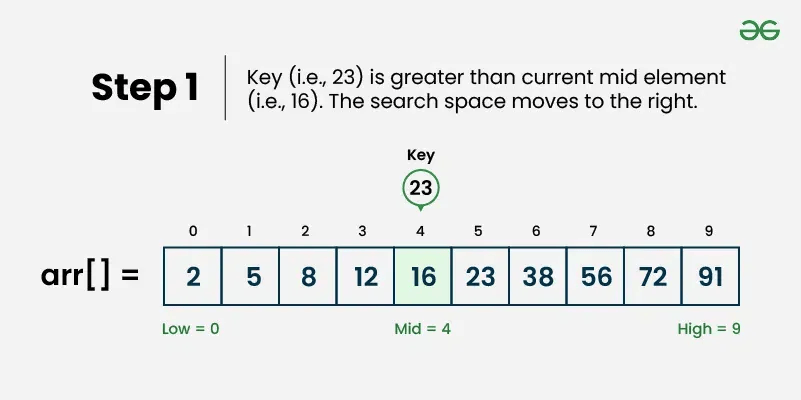
\includegraphics[scale=0.4]{images/Binary-Search-2.png} \\
    %\cite{BinarySearchGeeks}
    }
    \only<3>
    {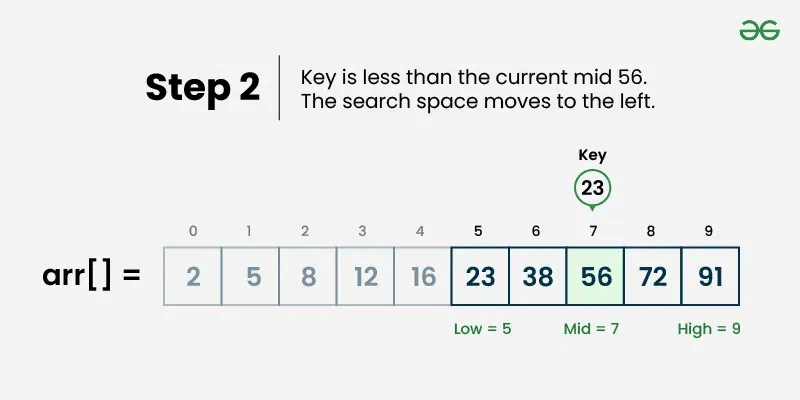
\includegraphics[scale=0.4]{images/Binary-Search-3.png} \\
    %\cite{BinarySearchGeeks}
    }
    \only<4>
    {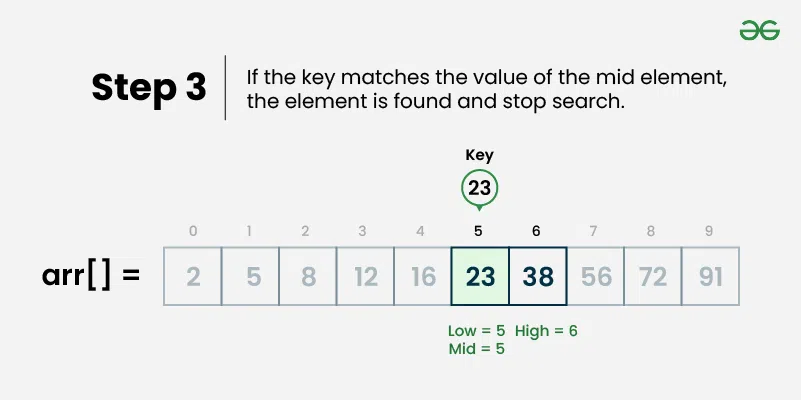
\includegraphics[scale=0.4]{images/Binary-Search-4.png} \\
    }
    %\cite{BinarySearchGeeks}
\end{frame}

% \begin{frame}{Show C++ Program}
%     Show C++ Program
% \end{frame}

\begin{frame}{Edge Case for Newton's Method}
    \begin{center}
        Use Newton's Method to solve $f(x) = \sqrt[3]{x}$
    \end{center}
    Let's choose an initial guess of 1 and a tolerance of 0.001
    \begin{itemize}
        \centering
        \item[]<1->
        $f'(x) = \frac{1}{3}x^{-\frac{2}{3}}, x_0 = 1$ \\
        \item[]<2->
        $x_1 = 1 - \frac{1^{\frac{1}{3}}}{\frac{1}{3}1^{-\frac{2}{3}}} = -2$
        \item[]<3->
        $x_2 = -2 - \frac{-2^{\frac{1}{3}}}{\frac{1}{3} \cdot -2^{-\frac{2}{3}}} = 4$
        \item[]<4->
        $x_3 = -8, x_4 = 16, x_5 = -32, x_k = (-2)^k$ \\ \vspace{0.3 cm}
    \end{itemize}
    \only<4->{When $f(x) = \sqrt[3]{x}$, Newton's method fails to find the solution of $x = 0$ when $x_0 \ne 0$.}
    % \begin{gather*}
    %     f(x) = x^3 - 0,f'(x) = 3x^2,  x_0 = 1\\
    %     x_{k+1} = \frac{1}{n} \left( x_k(n-1)+\frac{a}{x_k^{n-1}} \right) \\
    %     x_{1} = \frac{1}{3}\left( 1(3-1)+\frac{0}{1^{3-1}} \right) = \frac{2}{3} \\
    %     x_2 = \frac{1}{3}\left( \frac{2}{3}(3-1)+0 \right) = \frac{4}{9}\\ \\
    %     x_3 = \frac{1}{3}\left( \frac{4}{9}(3-1) \right) = \frac{8}{27} \\
    %     x_k = \frac{2^k}{3^k}
    % \end{gather*}
    \begin{center}
        %\cite{zeroExample}
    \end{center}
\end{frame}

% \begin{frame}{Show Edge Cases for Binary Search}
%     Show cases where Binary Search doesn't work.
% \end{frame}

% \begin{frame}{Conclusions}
    
% \end{frame}

% \begin{frame}{References}
%     % \footnotesize
%     %\bibliographystyle{apalike}
%     %\printbibliography
% \end{frame}

%------------------------------------------------

% \begin{frame}{Blocks of Highlighted Text}
%     In this slide, some important text will be \alert{highlighted} because it's important. Please, don't abuse it.

%     \begin{block}{Block}
%         Sample text
%     \end{block}

%     \begin{alertblock}{Alertblock}
%         Sample text in red box
%     \end{alertblock}

%     \begin{examples}
%         Sample text in green box. The title of the block is ``Examples".
%     \end{examples}
% \end{frame}

%------------------------------------------------

% \begin{frame}{Multiple Columns}
%     \begin{columns}[c] % The "c" option specifies centered vertical alignment while the "t" option is used for top vertical alignment

%         \column{.45\textwidth} % Left column and width
%         \textbf{Heading}
%         \begin{enumerate}
%             \item Statement
%             \item Explanation
%             \item Example
%         \end{enumerate}

%         \column{.45\textwidth} % Right column and width
%         Lorem ipsum dolor sit amet, consectetur adipiscing elit. Integer lectus nisl, ultricies in feugiat rutrum, porttitor sit amet augue. Aliquam ut tortor mauris. Sed volutpat ante purus, quis accumsan dolor.

%     \end{columns}
% \end{frame}

%------------------------------------------------
% \section{Second Section}
%------------------------------------------------

% \begin{frame}{Table}
%     \begin{table}
%         \begin{tabular}{l l l}
%             \toprule
%             \textbf{Treatments} & \textbf{Response 1} & \textbf{Response 2} \\
%             \midrule
%             Treatment 1         & 0.0003262           & 0.562               \\
%             Treatment 2         & 0.0015681           & 0.910               \\
%             Treatment 3         & 0.0009271           & 0.296               \\
%             \bottomrule
%         \end{tabular}
%         \caption{Table caption}
%     \end{table}
% \end{frame}

%------------------------------------------------

% \begin{frame}{Theorem}
%     \begin{theorem}[Mass--energy equivalence]
%         $E = mc^2$
%     \end{theorem}
% \end{frame}

%------------------------------------------------

% \begin{frame}{Figure}
%     Uncomment the code on this slide to include your own image from the same directory as the template .TeX file.
%     %\begin{figure}
%     %\includegraphics[width=0.8\linewidth]{test}
%     %\end{figure}
% \end{frame}

%------------------------------------------------

% \begin{frame}[fragile] % Need to use the fragile option when verbatim is used in the slide
%     \frametitle{Citation}
%     An example of the \verb|\cite| command to cite within the presentation:\\~

%     This statement requires citation \cite{p1}.
% \end{frame}

%------------------------------------------------

%------------------------------------------------

% \begin{frame}
%     \Huge{\centerline{\textbf{The End}}}
% \end{frame}

%----------------------------------------------------------------------------------------

\end{document}